\documentclass[tikz,border=10pt]{standalone}
\usepackage{tikz}
\usetikzlibrary{trees,shapes,positioning}

\begin{document}
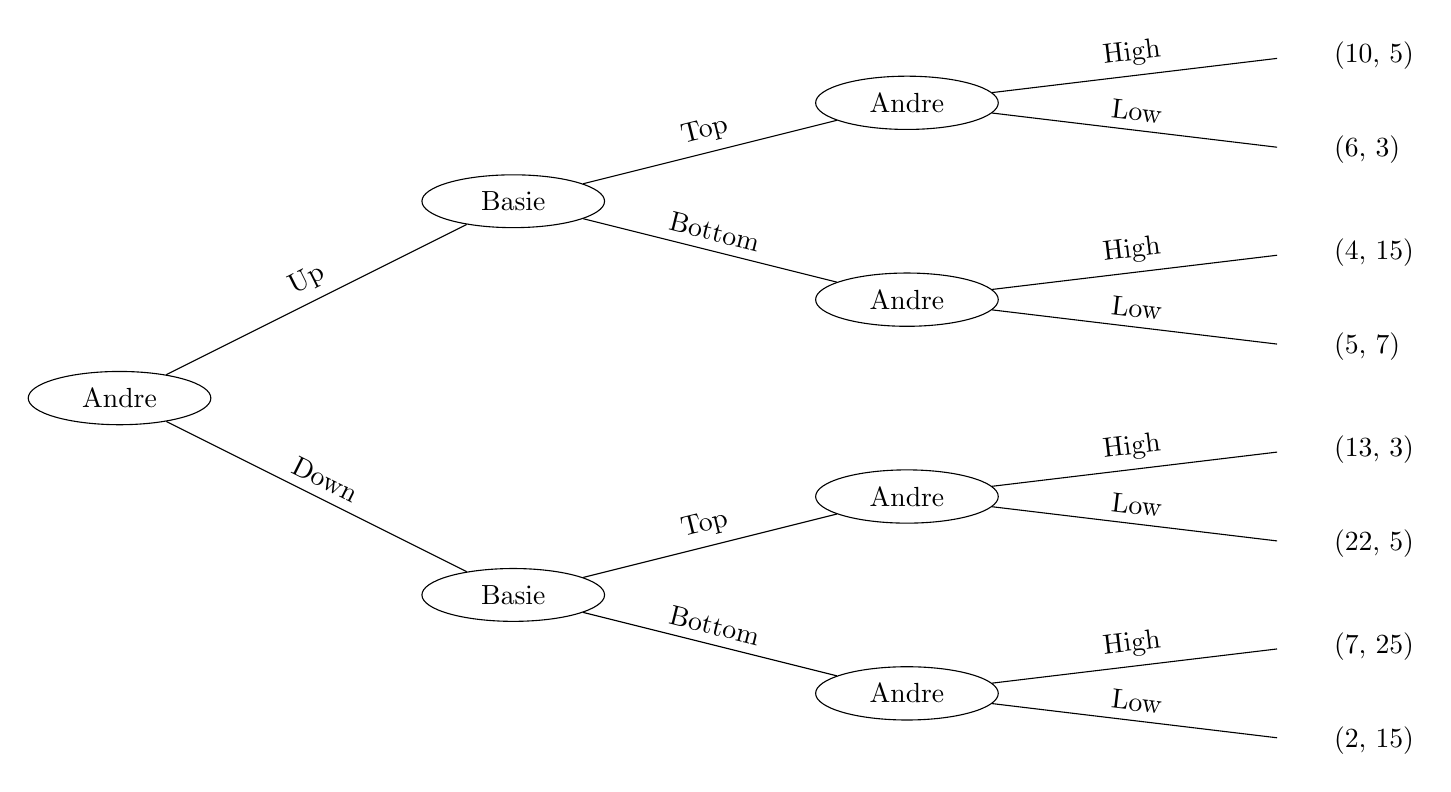
\begin{tikzpicture}[
  grow=right,
  sloped,
  level 1/.style={sibling distance=5cm, level distance=5cm},
  level 2/.style={sibling distance=2.5cm, level distance=5cm},
  level 3/.style={sibling distance=1.2cm, level distance=5cm},
  bag/.style={ellipse, draw, text width=4em, text centered},
  end/.style={text width=1em, text centered}
  ]
\node[bag] {Andre}
    child {
        node[bag] {Basie}        
            child {
                node[bag] {Andre} 
                        child {
                            node[end, label=right:
                                {(2, 15)}] {}
                            edge from parent
                            node[above] {Low}
                        }
                        child {
                            node[end, label=right:
                                {(7, 25)}] {}
                            edge from parent
                            node[above] {High}
                        }
                    edge from parent
                    node[above] {Bottom}
                }
            child {
                node[bag] {Andre} 
                    child {
                        node[end, label=right:
                            {(22, 5)}] {}
                        edge from parent
                        node[above] {Low}
                    }
                    child {
                        node[end, label=right:
                            {(13, 3)}] {}
                        edge from parent
                        node[above] {High}
                    }
                edge from parent
                node[above] {Top}
            }
        edge from parent         
        node[above] {Down}
    }
    child {
        node[bag] {Basie}        
            child {
                node[bag] {Andre}
                    child {
                        node[end, label=right:
                            {(5, 7)}] {}
                        edge from parent
                        node[above] {Low}
                    }
                    child {
                        node[end, label=right:
                            {(4, 15)}] {}
                        edge from parent
                        node[above] {High}
                    }
                edge from parent
                node[above] {Bottom}
            }
            child {
                node[bag] {Andre} 
                    child {
                        node[end, label=right:
                            {(6, 3)}] {}
                        edge from parent
                        node[above] {Low}
                    }
                    child {
                        node[end, label=right:
                            {(10, 5)}] {}
                        edge from parent
                        node[above] {High}
                    }
                edge from parent
                node[above] {Top}
            }
        edge from parent 
        node[above] {Up}
    };
\end{tikzpicture}
\end{document}
